% =====================================================================================
% Praesentations-Bausteine zur Auswertung INDEX320_cowfix-v1 (2026-06-18)
% Benoetigt: \usepackage{pgfplots}\pgfplotsset{compat=1.18}  und  \usepackage{booktabs}
% Quelle der Zahlen: analyze_ff.py -> ff_summary.json / tikz_data.csv  (nur two_phase_valid==1, MEDIAN).
% Hinweis: CLU-Werte werden BEWUSST nicht geplottet (Instrumentierung defekt, s. Auswertung).
% =====================================================================================

% -------------------------------------------------------------------------------------
% ABB. 1 — search_algo: staerkster cache-line-aware Hebel (absolute Median-Latenz)
% -------------------------------------------------------------------------------------
\begin{figure}[!htbp]\centering
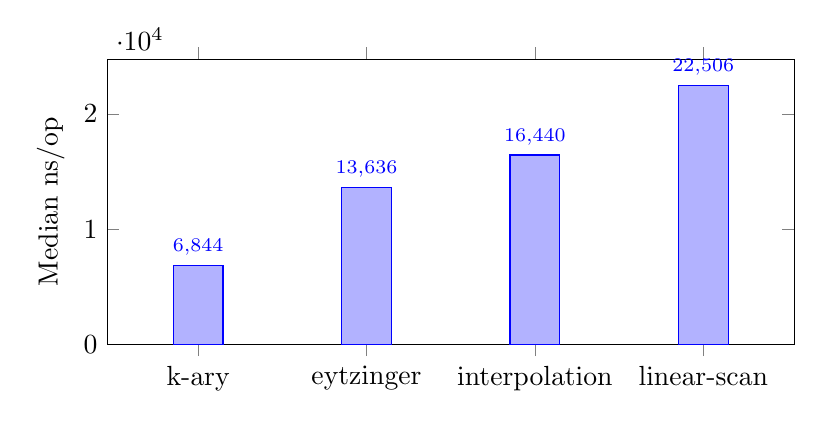
\begin{tikzpicture}
\begin{axis}[ybar, width=0.85\linewidth, height=5.2cm, ymin=0,
    ylabel={Median ns/op}, symbolic x coords={k-ary,eytzinger,interpolation,linear-scan},
    xtick=data, nodes near coords, nodes near coords style={font=\scriptsize},
    enlarge x limits=0.18, bar width=18pt]
\addplot coordinates {(k-ary,6844) (eytzinger,13636) (interpolation,16440) (linear-scan,22506)};
\end{axis}
\end{tikzpicture}
\caption{Such-Achse (marginal, alle Workloads): k-ary-Suche $-70\,\%$ gegenueber linearem Scan ---
der staerkste und robusteste cache-line-bewusste Effekt im Lauf.}\label{fig:msd-searchalgo}
\end{figure}

% -------------------------------------------------------------------------------------
% ABB. 2 — node_type: marginal vs. kontrolliert (relativ zum Besten = 1.0)
% Kernbotschaft: node256 konsistent am schlechtesten; node4 nur marginal schlecht (Schreib/Scan-Tiefe).
% -------------------------------------------------------------------------------------
\begin{figure}[!htbp]\centering
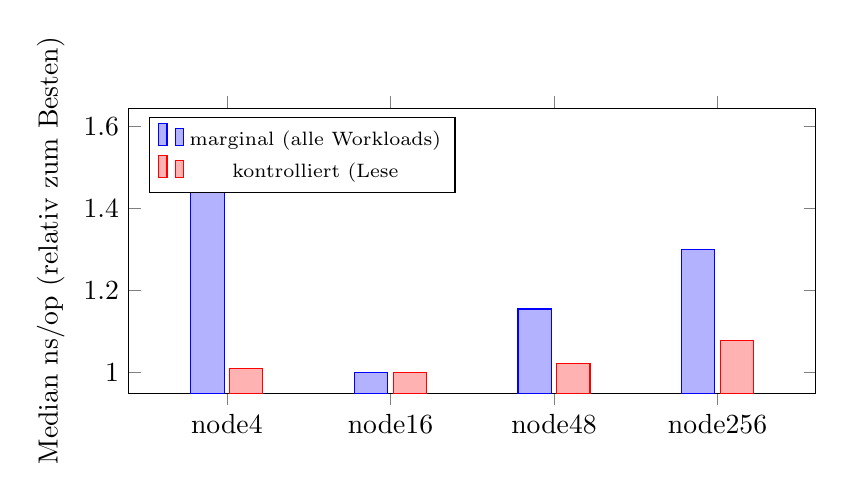
\begin{tikzpicture}
\begin{axis}[ybar, width=0.85\linewidth, height=5.2cm, ymin=0.95,
    ylabel={Median ns/op (relativ zum Besten)}, symbolic x coords={node4,node16,node48,node256},
    xtick=data, enlarge x limits=0.2, bar width=12pt, legend pos=north west, legend style={font=\scriptsize}]
\addplot coordinates {(node4,1.582) (node16,1.000) (node48,1.155) (node256,1.301)};
\addplot coordinates {(node4,1.010) (node16,1.000) (node48,1.023) (node256,1.079)};
\legend{marginal (alle Workloads), kontrolliert (Lese, k-ary)}
\end{axis}
\end{tikzpicture}
\caption{Knotentyp: node256 ist isoliert konsistent am teuersten (Cache-Line-Verschwendung);
node4 ist nur \emph{marginal} schlecht --- ein Baumtiefen-Artefakt schreib-/scan-lastiger Lasten,
nicht der Lese-Latenz. Sweet-Spot node16.}\label{fig:msd-nodetype}
\end{figure}

% -------------------------------------------------------------------------------------
% ABB. 3 — memory_layout: der "ehrliche" Befund (Effekt verschwindet unter Kontrolle)
% -------------------------------------------------------------------------------------
\begin{figure}[!htbp]\centering
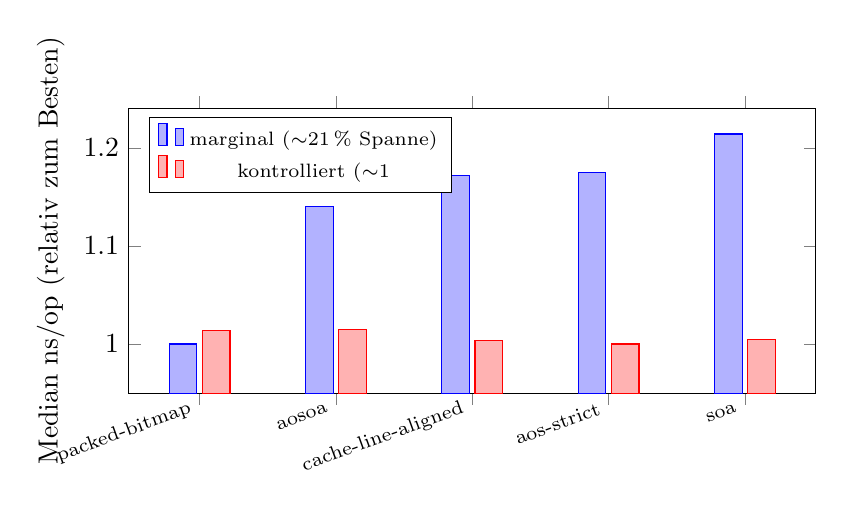
\begin{tikzpicture}
\begin{axis}[ybar, width=0.85\linewidth, height=5.2cm, ymin=0.95,
    ylabel={Median ns/op (relativ zum Besten)},
    symbolic x coords={packed-bitmap,aosoa,cache-line-aligned,aos-strict,soa},
    xtick=data, x tick label style={rotate=20,anchor=east,font=\scriptsize},
    enlarge x limits=0.13, bar width=10pt, legend pos=north west, legend style={font=\scriptsize}]
\addplot coordinates {(packed-bitmap,1.000) (aosoa,1.140) (cache-line-aligned,1.172) (aos-strict,1.175) (soa,1.214)};
\addplot coordinates {(packed-bitmap,1.014) (aosoa,1.015) (cache-line-aligned,1.004) (aos-strict,1.000) (soa,1.005)};
\legend{marginal ($\sim$21\,\% Spanne), kontrolliert ($\sim$1,5\,\% Spanne)}
\end{axis}
\end{tikzpicture}
\caption{Speicher-Layout (Kern der ``cache-line-aware''-Idee): Der scheinbare marginale Vorteil
($\sim$21\,\%) ist Konfundierung --- unter Kontrolle bleiben nur $\sim$1,5\,\%. \textbf{Kein robuster
Layout-Vorteil nachgewiesen}; die eigentliche CLU-Kennzahl ist zudem defekt.}\label{fig:msd-layout}
\end{figure}

% -------------------------------------------------------------------------------------
% ABB. 4 — prefetch: kein Nutzen (marginal leichte Verschlechterung, kontrolliert Patt)
% -------------------------------------------------------------------------------------
\begin{figure}[!htbp]\centering
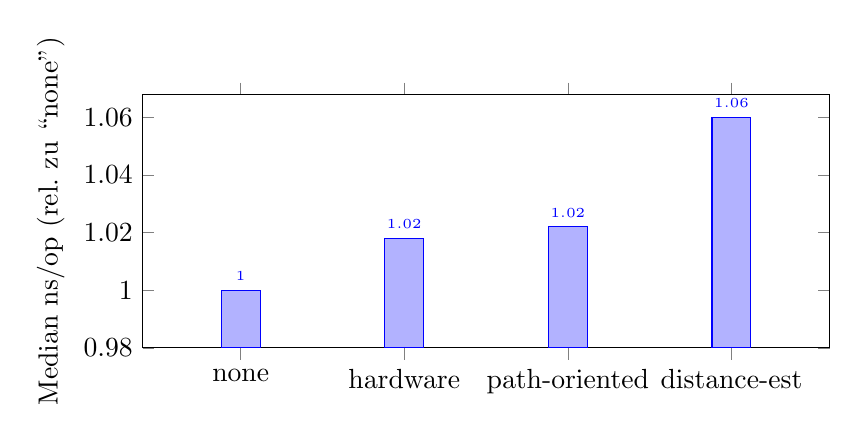
\begin{tikzpicture}
\begin{axis}[ybar, width=0.85\linewidth, height=4.8cm, ymin=0.98,
    ylabel={Median ns/op (rel.\ zu ``none'')}, symbolic x coords={none,hardware,path-oriented,distance-est},
    xtick=data, nodes near coords, nodes near coords style={font=\tiny},
    enlarge x limits=0.2, bar width=14pt]
\addplot coordinates {(none,1.000) (hardware,1.018) (path-oriented,1.022) (distance-est,1.060)};
\end{axis}
\end{tikzpicture}
\caption{Prefetch-Achse (marginal): kein Organ schlaegt ``kein Prefetch''. Bei in-Cache-Arbeitssatz
reiner Overhead; kontrolliert ist der Unterschied ein Patt ($\sim$2\,\%).}\label{fig:msd-prefetch}
\end{figure}

% -------------------------------------------------------------------------------------
% ABB. 5 — Workload-Spanne (Median ns/op, log-Skala) — erklaert die Ausreisser-Herkunft
% -------------------------------------------------------------------------------------
\begin{figure}[!htbp]\centering
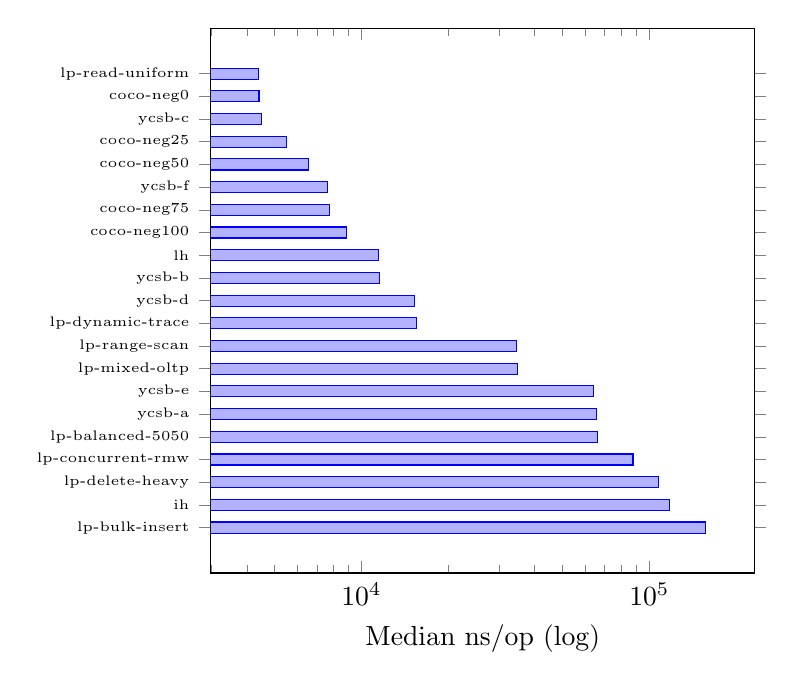
\begin{tikzpicture}
\begin{axis}[xbar, width=0.7\linewidth, height=8.5cm, xmode=log, xmin=3000,
    xlabel={Median ns/op (log)}, symbolic y coords={%
      lp-bulk-insert,ih,lp-delete-heavy,lp-concurrent-rmw,lp-balanced-5050,ycsb-a,ycsb-e,%
      lp-mixed-oltp,lp-range-scan,lp-dynamic-trace,ycsb-d,ycsb-b,lh,coco-neg100,coco-neg75,%
      ycsb-f,coco-neg50,coco-neg25,ycsb-c,coco-neg0,lp-read-uniform},
    ytick=data, y tick label style={font=\tiny}, bar width=4pt]
\addplot coordinates {(156402,lp-bulk-insert) (117701,ih) (108010,lp-delete-heavy) (87767,lp-concurrent-rmw)
 (66078,lp-balanced-5050) (65652,ycsb-a) (64105,ycsb-e) (34880,lp-mixed-oltp) (34508,lp-range-scan)
 (15508,lp-dynamic-trace) (15344,ycsb-d) (11588,ycsb-b) (11470,lh) (8857,coco-neg100) (7732,coco-neg75)
 (7606,ycsb-f) (6548,coco-neg50) (5480,coco-neg25) (4484,ycsb-c) (4409,coco-neg0) (4379,lp-read-uniform)};
\end{axis}
\end{tikzpicture}
\caption{21 Workloads, Median ns/op (log): $\sim$36$\times$ Spanne. Die schweren Schreib-/Scan-/Bulk-Lasten
oben erzeugen den rechten Tail (9\,\% Ausreisser $>10\times$ Median) --- groesstenteils \emph{echte} Kosten,
keine reinen Mess-Artefakte.}\label{fig:msd-workloads}
\end{figure}

% -------------------------------------------------------------------------------------
% TAB. 1 — Achsen-Effekte kompakt (marginal vs. kontrolliert)
% -------------------------------------------------------------------------------------
\begin{table}[!htbp]\centering\small
\caption{Achsen-Effekte auf die Median-Latenz (ns/op). Kontrolliert = Lese-Workloads, search\_algo=k-ary.}
\label{tab:msd-axes}
\begin{tabular}{@{}llrr@{}}
\toprule
Achse & bester $\to$ schlechtester & Spanne marginal & Spanne kontrolliert \\
\midrule
search\_algo   & k-ary $\to$ linear-scan      & $+229\,\%$ & (fixiert) \\
node\_type     & node16 $\to$ node256        & $+58\,\%$  & $+7{,}9\,\%$ \\
memory\_layout & (kein robuster Gewinner)    & $+21\,\%$  & $+1{,}5\,\%$ \\
prefetch       & none $\to$ distance-est     & $+6\,\%$   & $+2{,}1\,\%$ (Patt) \\
\bottomrule
\end{tabular}
\end{table}

% -------------------------------------------------------------------------------------
% TAB. 2 — Forschungsfragen: ableitbare Tendenzen aus dem (buggy) Lauf
% -------------------------------------------------------------------------------------
\begin{table}[!htbp]\centering\small
\caption{Aus dem Messlauf ableitbare FF-Tendenzen (Stand: bekannte Instrumentierungs-Defekte).}
\label{tab:msd-ff}
\begin{tabular}{@{}l>{\raggedright\arraybackslash}p{8.2cm}l@{}}
\toprule
FF & Tendenz & Aussagekraft \\
\midrule
FF0 & Aktiv cache-bewusste \emph{Suche} (k-ary) bringt $-70\,\%$; Layout/Prefetch zeigen \emph{keinen} Nutzen; Plattform-Variation nicht testbar (nur amd64). & teilweise \\
FF1 & Orthogonale Permutationsmatrix (320 = $5\times4\times4\times4$) bestaetigt; starke Achse$\times$Workload-Kopplung (node4 kippt); SIMD-Kopplung nicht testbar. & ja (Komposition) \\
FF2 & Knotengroessen-Streit: kleine Knoten besser, Sweet-Spot node16, node256 schlechtester; Pipeline valide, aber CLU-Bug + 9\,\% Tail. & teilweise \\
FF3 & \emph{Nicht} beantwortbar: kein PRT-ART/SOTA-Lebewesen im Lauf; CLU/LLC/dTLB fehlen bzw.\ defekt. & offen \\
FF4 & Compile-Time-Achsen dominieren + sind provenienz-codiert; Laufzeit (thread\_count=3, prefetch\_distance=2) nur teil-gesweept. & teilweise \\
\bottomrule
\end{tabular}
\end{table}
